% !TEX encoding = UTF-8 Unicode

\documentclass[a4paper]{article}

\usepackage{color}
\usepackage{url}
\usepackage[T2A]{fontenc} % enable Cyrillic fonts
\usepackage[utf8]{inputenc} % make weird characters work
\usepackage{graphicx}

\usepackage[english,serbian]{babel}
%\usepackage[english,serbianc]{babel} %ukljuciti babel sa ovim opcijama, umesto gornjim, ukoliko se koristi cirilica

\usepackage[unicode]{hyperref}
\hypersetup{colorlinks,citecolor=green,filecolor=green,linkcolor=blue,urlcolor=blue}

%\newtheorem{primer}{Пример}[section] %ćirilični primer
\newtheorem{primer}{Primer}[section]

\begin{document}

\title{Klimatske promene - mit ili realnost\\ \small{Seminarski rad u okviru kursa\\Tehničko i naučno pisanje\\ Matematički fakultet}}


\author{Ana Šaponjić\\ mi21255@alas.matf.bg.ac.rs \and Elena Zorić\\ mi21300@alas.matf.bg.ac.rs \and Marija Trišović\\ mi21164@alas.matf.bg.ac.rs\and \\Mihajlo Živanović\\ mi21353@alas.matf.bg.ac.rs }
\date{1.~decembar 2022.}


\date{decembar 2022.}
\maketitle
\abstract{
 \footnotesize {
 U ovom tekstu je ukratko objašnjeno šta su  klimatske promene. Kako one utiču na na promene flore  i faune, ali ne samo toga nego i mnogih promena koje mogu dovesti do potpune promene reljefa, takođe koje su posledice svih klimatskih promena i šta one prouzrokuju. Samim tim  ova tema poteže mnogo pitanja. Šta je uzrok, pitanje na koje se daju različiti odgovori.}}

\tableofcontents

\newpage

\section{Uvod}
\label{sec:uvod}
Termin klimatske promene, se do industrijske revolucije je bio vezan za rezultat promena prirodnih okolnosti. Međutim danas termin klimatske promene koristimo kada govorimo o promenama klime od početka dvadesetog veka, koje su nastale kao posledica ljudskih aktivnosti.


Klimatske promene, posebno one koje su u opticaju globalnog zagrevanja, postaju ozbiljnim problemom za prirodu i ljudsko društvo. Njihove posledice su očigledne kada su u pitanju biodiverzitet, biljne i životinjske vrste, pa i čovek. Temperature rastu, i topi led ma polovima, samim tim se nivo mora povećava , što utiče na floru i faunu na priobalnom području zvoj 
Mišljenje stručnjaka je podeljno. Jedni misle da su ove promene samo deo razvoja planete i da je čovekov uticaj jako mali.




\section{Topljenje glečera}
\label{sec:toplenje_glečera}
Globalno zagrevanje će dovoditi do rasta nivoa mora usled topljenja leda, a taj porast nivoa mora može trajati čitav milenijum .Klimatske promene predstavljaju „primarni ekološki izazov“ prvog veka trećeg milenijuma. Istraživanja Grenlanda su pokazala da je glečer 2012. ušao u fazu nestajanja i završavanja leda u vodama severnog Atlantika. Ipak se leti otopi veća količina leda od one koja se ne može nadoknaditi zimi. To dovodi do toga da se manje sunčeve svetlosti odbija od površinu okeana, voda više apsorbuje toplotu i postaje toplija.

Na Antarktiku je primijećena džinovska rupa za koju naučnici tvrde da je rascjep ledene površine veći od teritorije Holandije. Zato uporno ukazuju na moguću kataklizmu – Arktik bez leda do 2040. godine.
Ukoliko bi se to dogodilo, to bi značilo da bi Arktik postao velikim vodenim područjem koje bi promijenilo floru i faunu, biodiverzitet i ekosisteme. Naravno, u takvoj situaciji nestale bi 20 mnoge biljne i životinjske vrste kao što su, na primer, foke i polarni medvedi. Pretpostavlja se da bi, zbog klimatskih promena, u slijedećih nekoliko decenija moglo doći do izumiranja polarnih medveda.

\begin{figure}[!ht]
\begin{center}
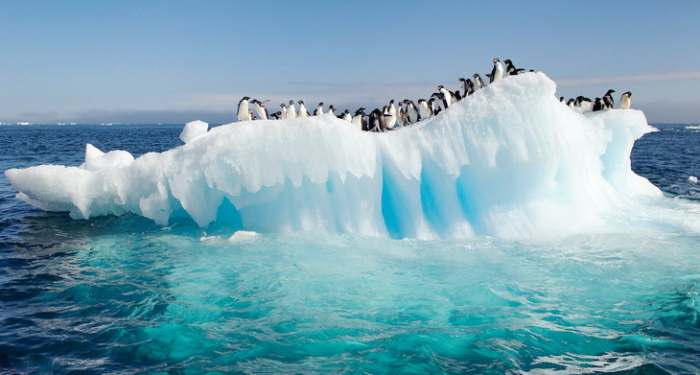
\includegraphics[scale=0.5]{slika2.jpg}
\end{center}
\caption{Topljenje glečera}
\label{fig:glecer}
\end{figure}

\section{Promene klimatskih obrazaca
i elementarne nepogode}	
\label{sec:promene_klimatskih_obrazaca}
Ono što je sada već poznato jeste da suvi regioni postati još suvlji. To znači da u regionima koje imaju malo padavina će biti sve manje, dok će regioni  koji su vlažni iskusiti povećanje padavina. 
Brojnim istraživanjima je dokazano jeste da padavine traju kraće ali da su intenzivije. Na primer umesto da padavina traje nedelju dana umerenim intezitetom, za 2 dana će pasti ista količina padavina. To dovodi do povećanog rizika od poplava.

Naučnici su ipak jasno upozorili da jedan klimatski poremećaj ne može da se pripiše samo ekstremnim posledicama klimatskih promena globalnog zagrevanja dovode do velikih oscilacija u temperaturama. Samo u 2014. godini ih je bilo pogođeno 39,7 miliona, u poplavama 36,6 i u olujama 25,7 miliona. Pod uticajem globalnog zagrevanja, javljaju se velike vrućine čije temperature stvaraju  požare.

Klimatske promene sa svojim promenjenim klimatskim obrascima prouzrokuju izumiranje nekih biljnih i životinjskih vrsta. 

\section{Efekat staklene bašte}	
\label{sec:efekat_staklene_baste}
Efekat staklene bašte je proces zagrevanja Zemlje koji je nastao poremećajem energetske ravnoteže između količine zračenja koje Zemljina površina prima od Sunca i vraća u svemir. Deo toplotnog zračenja, koje stiže do Zemljine kore, odbija se u atmosferu i, umesto da ode u svemir, apsorbuju ga neki gasovi u atmosferi i ponovno dozračuju na Zemlju. Na ovaj način se temperatura Zemljine površine povišava.

\begin{figure}[!ht]
\begin{center}
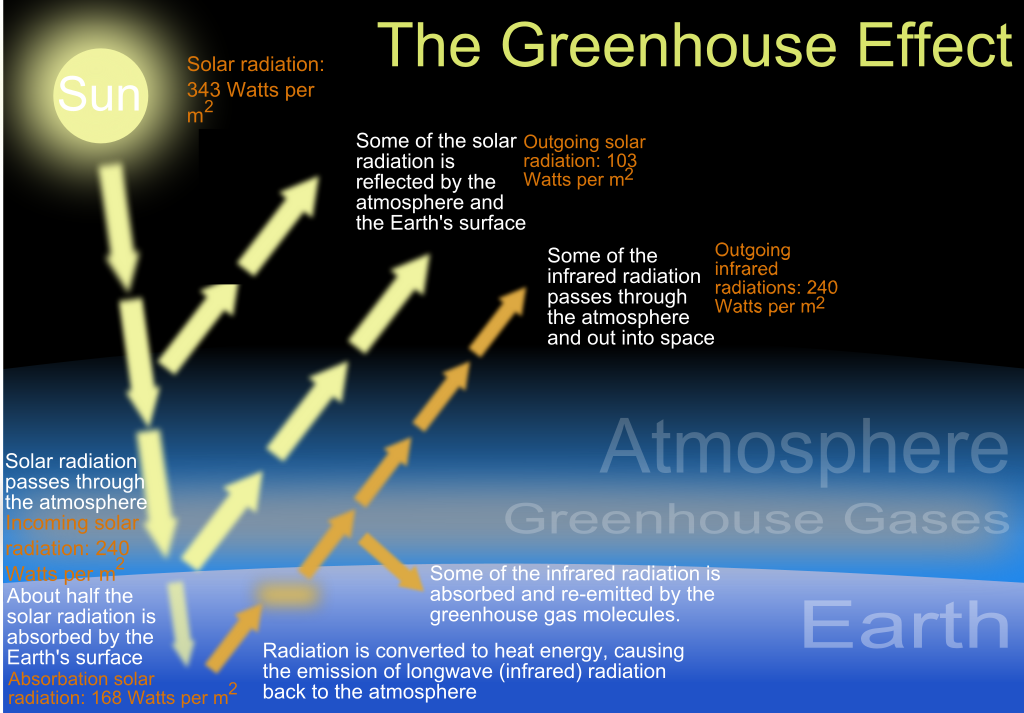
\includegraphics[scale=0.26]{slika3.png}
\end{center}
\caption{Efekat staklene bašte}
\label{fig:efekat}
\end{figure}

\end{document}
